\documentclass[12pt,a4paper]{article}
\usepackage[utf8]{inputenc}
\usepackage{amsmath}
\usepackage{amsfonts}
\usepackage{amssymb}
\usepackage{graphicx}
\usepackage{tikz}
\usetikzlibrary{automata,positioning,arrows.meta,shapes,trees}
\usepackage{geometry}
\usepackage{listings}
\usepackage{xcolor}
\usepackage{fancyhdr}
\usepackage{hyperref}
\usepackage{tabularx}
\usepackage{syntax}

\geometry{margin=1in}
\pagestyle{fancy}
\fancyhf{}
\rhead{YACC/Bison Theory}
\lhead{Assignment 03 v1}
\cfoot{\thepage}

% Code listing style
\lstset{
    language=C,
    basicstyle=\ttfamily\small,
    keywordstyle=\color{blue},
    commentstyle=\color{green!60!black},
    stringstyle=\color{red},
    numbers=left,
    numberstyle=\tiny,
    breaklines=true,
    frame=single,
    tabsize=4
}

\title{\textbf{Syntax Analysis using YACC/Bison}\\
\large{Assignment 03 Version 1 - Theoretical Documentation}}
\author{Compiler Design Laboratory}
\date{\today}

\begin{document}

\maketitle

\tableofcontents
\newpage

\section{Introduction}

This document provides comprehensive theoretical documentation for the syntax analyzer (parser) implementation using YACC/Bison in Assignment 03 Version 1.

\subsection{What is Syntax Analysis?}

Syntax analysis is the second phase of compilation:
\begin{itemize}
    \item \textbf{Input}: Token stream from lexical analyzer
    \item \textbf{Process}: Check grammatical structure
    \item \textbf{Output}: Parse tree or abstract syntax tree
    \item \textbf{Error Detection}: Report syntax errors
\end{itemize}

\subsection{Compiler Pipeline}

\begin{figure}[h!]
\centering
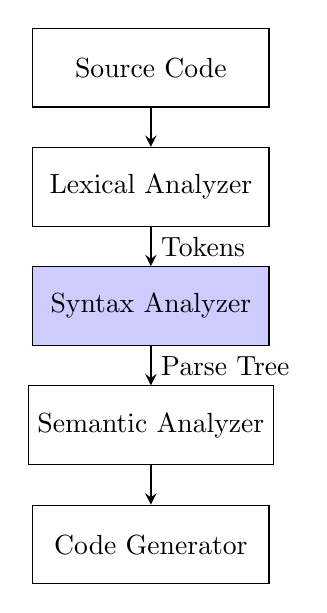
\begin{tikzpicture}[
    box/.style={rectangle, draw, minimum width=3cm, minimum height=1cm},
    arrow/.style={->, >=stealth, thick}
]
    \node[box] (source) {Source Code};
    \node[box, below=0.5cm of source] (lex) {Lexical Analyzer};
    \node[box, below=0.5cm of lex, fill=blue!20] (syn) {Syntax Analyzer};
    \node[box, below=0.5cm of syn] (sem) {Semantic Analyzer};
    \node[box, below=0.5cm of sem] (icg) {Code Generator};
    
    \draw[arrow] (source) -- (lex);
    \draw[arrow] (lex) -- node[right] {Tokens} (syn);
    \draw[arrow] (syn) -- node[right] {Parse Tree} (sem);
    \draw[arrow] (sem) -- (icg);
\end{tikzpicture}
\caption{Syntax Analyzer in Compiler Pipeline}
\end{figure}

\section{Context-Free Grammars}

\subsection{Formal Definition}

A Context-Free Grammar (CFG) is a 4-tuple $G = (V, T, P, S)$:
\begin{itemize}
    \item $V$: Finite set of non-terminal symbols
    \item $T$: Finite set of terminal symbols (tokens)
    \item $P$: Finite set of production rules: $A \rightarrow \alpha$ where $A \in V$ and $\alpha \in (V \cup T)^*$
    \item $S$: Start symbol, $S \in V$
\end{itemize}

\subsection{Example Grammar}

\textbf{C Subset Grammar:}

\begin{align*}
\text{program} &\rightarrow \text{main\_function} \\
\text{main\_function} &\rightarrow \text{INT\_TOK ID\_TOK LPAREN\_TOK RPAREN\_TOK compound\_statement} \\
\text{compound\_statement} &\rightarrow \text{LBRACE\_TOK statement\_list RBRACE\_TOK} \\
\text{statement\_list} &\rightarrow \text{statement\_list statement} \mid \varepsilon \\
\text{statement} &\rightarrow \text{assignment\_statement} \mid \text{conditional\_statement}
\end{align*}

\subsection{Derivations}

\textbf{Leftmost Derivation:} Always expand leftmost non-terminal first

\textbf{Example:} Derive \texttt{int main() \{ x = 10; \}}

\begin{align*}
\text{program} &\Rightarrow \text{main\_function} \\
&\Rightarrow \text{INT\_TOK ID\_TOK LPAREN\_TOK RPAREN\_TOK compound\_statement} \\
&\Rightarrow \text{INT\_TOK ID\_TOK LPAREN\_TOK RPAREN\_TOK LBRACE statement\_list RBRACE} \\
&\Rightarrow \ldots
\end{align*}

\subsection{Parse Trees}

\begin{figure}[h!]
\centering
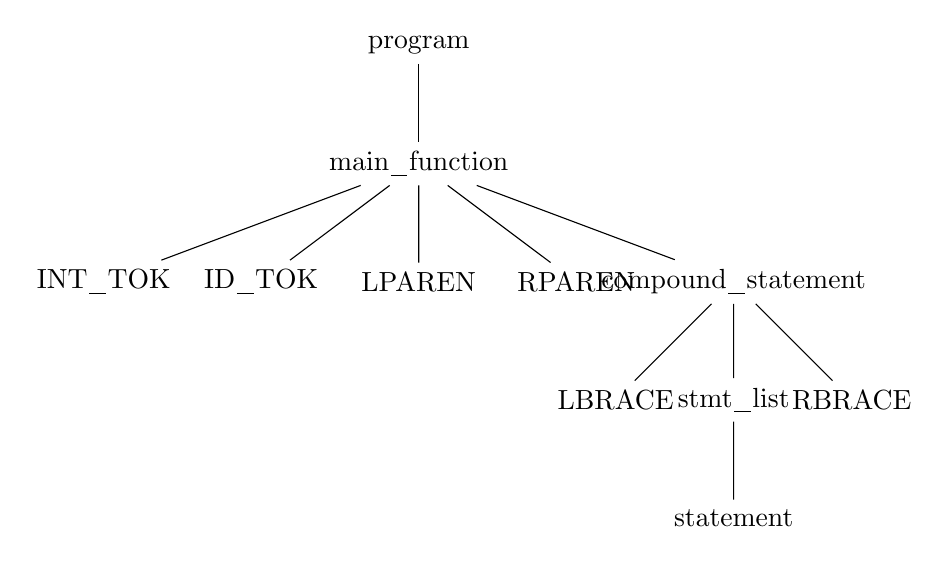
\begin{tikzpicture}[
    level 1/.style={sibling distance=4cm},
    level 2/.style={sibling distance=2cm},
    level 3/.style={sibling distance=1.5cm}
]
\node {program}
    child {node {main\_function}
        child {node {INT\_TOK}}
        child {node {ID\_TOK}}
        child {node {LPAREN}}
        child {node {RPAREN}}
        child {node {compound\_statement}
            child {node {LBRACE}}
            child {node {stmt\_list}
                child {node {statement}}
            }
            child {node {RBRACE}}
        }
    };
\end{tikzpicture}
\caption{Parse Tree Example}
\end{figure}

\section{Parsing Algorithms}

\subsection{Top-Down vs Bottom-Up}

\begin{table}[h!]
\centering
\begin{tabularx}{\textwidth}{|l|X|X|}
\hline
\textbf{Aspect} & \textbf{Top-Down} & \textbf{Bottom-Up} \\
\hline
Direction & Start symbol $\rightarrow$ input & Input $\rightarrow$ start symbol \\
\hline
Derivation & Leftmost & Rightmost (reverse) \\
\hline
Examples & LL(1), Recursive Descent & LR(0), SLR(1), LALR(1), LR(1) \\
\hline
Power & Less powerful & More powerful \\
\hline
Error Handling & Better & Good \\
\hline
\end{tabularx}
\caption{Comparison of Parsing Strategies}
\end{table}

\subsection{LALR(1) Parsing}

YACC generates LALR(1) parsers:
\begin{itemize}
    \item \textbf{L}: Left-to-right scan of input
    \item \textbf{A}: Reversed rightmost derivation
    \item \textbf{LR}: Left-to-right, rightmost
    \item \textbf{(1)}: One token lookahead
\end{itemize}

\subsection{Parse Table Construction}

\textbf{LALR(1) Parse Table Components:}

\begin{enumerate}
    \item \textbf{ACTION Table}: $\text{ACTION}[s, a]$ where $s$ is state, $a$ is terminal
        \begin{itemize}
            \item \texttt{shift n}: Shift and go to state $n$
            \item \texttt{reduce A → α}: Reduce by production
            \item \texttt{accept}: Accept input
            \item \texttt{error}: Syntax error
        \end{itemize}
    
    \item \textbf{GOTO Table}: $\text{GOTO}[s, A]$ where $s$ is state, $A$ is non-terminal
        \begin{itemize}
            \item State to go to after reducing by $A$
        \end{itemize}
\end{enumerate}

\subsection{Parsing Example}

\textbf{Grammar:}
\begin{align*}
E &\rightarrow E + T \\
E &\rightarrow T \\
T &\rightarrow \text{ID}
\end{align*}

\textbf{Input:} \texttt{x + y}

\begin{table}[h!]
\centering
\small
\begin{tabular}{|l|l|l|}
\hline
\textbf{Stack} & \textbf{Input} & \textbf{Action} \\
\hline
\$ & \texttt{x + y \$} & shift \\
\$ \texttt{x} & \texttt{+ y \$} & reduce $T \rightarrow \text{ID}$ \\
\$ T & \texttt{+ y \$} & reduce $E \rightarrow T$ \\
\$ E & \texttt{+ y \$} & shift \\
\$ E + & \texttt{y \$} & shift \\
\$ E + \texttt{y} & \texttt{\$} & reduce $T \rightarrow \text{ID}$ \\
\$ E + T & \texttt{\$} & reduce $E \rightarrow E + T$ \\
\$ E & \texttt{\$} & accept \\
\hline
\end{tabular}
\caption{LALR Parsing Example}
\end{table}

\section{YACC Specification}

\subsection{Three-Section Structure}

\begin{lstlisting}
%{
/* Declarations section */
#include <stdio.h>
int syntax_errors = 0;
%}

/* Token and type declarations */
%token INT_TOK FLOAT_TOK ID_TOK

%%
/* Grammar rules section */
program: main_function
       { printf("Valid program\n"); }
       ;

main_function: INT_TOK ID_TOK LPAREN_TOK RPAREN_TOK
               compound_statement
             ;

%%
/* C code section */
int main() {
    yyparse();
    return 0;
}

void yyerror(const char *msg) {
    fprintf(stderr, "Error: %s\n", msg);
}
\end{lstlisting}

\subsection{Token Declarations}

\begin{lstlisting}
%token INT_TOK FLOAT_TOK CHAR_TOK
%token ID_TOK INTCONST_TOK FLOATCONST_TOK
%token ASSIGN_TOK ADD_TOK SUB_TOK MUL_TOK
%token LPAREN_TOK RPAREN_TOK LBRACE_TOK RBRACE_TOK
%token SEMICOLON_TOK
\end{lstlisting}

\subsection{Operator Precedence}

\begin{lstlisting}
%left OR_TOK
%left AND_TOK
%left BIT_OR_TOK
%left BIT_XOR_TOK
%left BIT_AND_TOK
%left EQ_TOK NEQ_TOK
%left LT_TOK GT_TOK LE_TOK GE_TOK
%left BIT_LSHIFT_TOK BIT_RSHIFT_TOK
%left ADD_TOK SUB_TOK
%left MUL_TOK DIV_TOK MOD_TOK
%right ASSIGN_TOK
%right NOT_TOK BIT_NOT_TOK
%left INC_TOK DEC_TOK
\end{lstlisting}

\textbf{Precedence Levels:} Lower declarations have higher precedence

\textbf{Associativity:}
\begin{itemize}
    \item \texttt{\%left}: Left associative (e.g., \texttt{a + b + c} = \texttt{(a + b) + c})
    \item \texttt{\%right}: Right associative (e.g., \texttt{a = b = c} = \texttt{a = (b = c)})
\end{itemize}

\section{Grammar Rules}

\subsection{Production Rule Syntax}

\textbf{Format:}
\begin{lstlisting}
non_terminal: symbol_1 symbol_2 ... symbol_n
            { action }
            | alternative_1 alternative_2
            { action }
            ;
\end{lstlisting}

\subsection{Semantic Actions}

\textbf{Value Stack:}
\begin{itemize}
    \item \texttt{\$\$}: Value of LHS non-terminal
    \item \texttt{\$1, \$2, ..., \$n}: Values of RHS symbols
\end{itemize}

\textbf{Example:}
\begin{lstlisting}
expression: expression ADD_TOK expression
          {
              $$ = $1 + $3;  // Compute sum
          }
          | INTCONST_TOK
          {
              $$ = $1;  // Pass constant value
          }
          ;
\end{lstlisting}

\subsection{Main Function Production}

\begin{lstlisting}
main_function: data_type ID_TOK LPAREN_TOK RPAREN_TOK 
               compound_statement
             {
                 printf("SYNTAX OK: Main function\n");
                 $$ = create_function($1, $2, NULL, $5);
             }
             | data_type ID_TOK LPAREN_TOK parameter_list 
               RPAREN_TOK compound_statement
             {
                 printf("SYNTAX OK: Main with parameters\n");
                 $$ = create_function($1, $2, $4, $6);
             }
             ;
\end{lstlisting}

\subsection{Statement Productions}

\begin{lstlisting}
statement: expression_statement
         | compound_statement
         | conditional_statement
         | iterative_statement
         | return_statement
         | assignment_statement
         ;

assignment_statement: ID_TOK ASSIGN_TOK expression SEMICOLON_TOK
                    {
                        printf("SYNTAX OK: Assignment\n");
                        $$ = make_assign($1, $3);
                    }
                    ;

conditional_statement: IF_TOK LPAREN_TOK expression RPAREN_TOK 
                      statement
                     {
                         $$ = make_if($3, $5, NULL);
                     }
                     | IF_TOK LPAREN_TOK expression RPAREN_TOK 
                       statement ELSE_TOK statement
                     {
                         $$ = make_if($3, $5, $7);
                     }
                     ;
\end{lstlisting}

\section{Error Handling}

\subsection{Error Detection}

\textbf{Automatic:} YACC detects syntax errors when no parse action is possible

\textbf{Error Token:}
\begin{lstlisting}
statement: error SEMICOLON_TOK
         {
             yyerrok;  // Resume parsing
             printf("ERROR: Invalid statement\n");
         }
         ;
\end{lstlisting}

\subsection{yyerror Function}

\begin{lstlisting}
void yyerror(const char *msg) {
    fprintf(stderr, "SYNTAX ERROR (Line %d): %s\n", 
            yylineno, msg);
    syntax_error_count++;
}
\end{lstlisting}

\subsection{Error Recovery Strategies}

\begin{enumerate}
    \item \textbf{Panic Mode}: Skip to synchronizing token
        \begin{lstlisting}
statement: error SEMICOLON_TOK { yyerrok; }
        \end{lstlisting}
    
    \item \textbf{Phrase-Level}: Insert/delete tokens locally
        \begin{lstlisting}
declaration: data_type error SEMICOLON_TOK
           { yyerror("Invalid declarator"); }
        \end{lstlisting}
    
    \item \textbf{Error Productions}: Explicit error rules
        \begin{lstlisting}
if_statement: IF_TOK error THEN_TOK statement
            { yyerror("Missing condition"); }
        \end{lstlisting}
\end{enumerate}

\section{Integration with Lexer}

\subsection{Token Communication}

\textbf{Shared Definitions:}

\texttt{parser.y} generates \texttt{parser.tab.h}:
\begin{lstlisting}
#define INT_TOK 258
#define FLOAT_TOK 259
#define ID_TOK 260
#define INTCONST_TOK 261
...
\end{lstlisting}

\textbf{Lexer includes header:}
\begin{lstlisting}
/* lex.l */
%{
#include "parser.tab.h"
%}

%%
"int"       { return INT_TOK; }
[a-zA-Z_]+  { yylval.sval = strdup(yytext); 
              return ID_TOK; }
[0-9]+      { yylval.ival = atoi(yytext); 
              return INTCONST_TOK; }
%%
\end{lstlisting}

\subsection{Semantic Values}

\textbf{Union Declaration:}
\begin{lstlisting}
%union {
    int ival;
    float fval;
    char *sval;
    struct node *nval;
}

%token <sval> ID_TOK
%token <ival> INTCONST_TOK
%token <fval> FLOATCONST_TOK
%type <nval> statement expression
\end{lstlisting}

\section{Parse Tree Construction}

\subsection{AST Node Structure}

\begin{lstlisting}
typedef struct node {
    enum { OP_NODE, ID_NODE, CONST_NODE } type;
    union {
        struct {
            char *op;
            struct node *left;
            struct node *right;
        } op_node;
        struct {
            char *name;
        } id_node;
        struct {
            int value;
        } const_node;
    } data;
} Node;
\end{lstlisting}

\subsection{Node Creation Functions}

\begin{lstlisting}
Node* make_op_node(char *op, Node *left, Node *right) {
    Node *n = malloc(sizeof(Node));
    n->type = OP_NODE;
    n->data.op_node.op = strdup(op);
    n->data.op_node.left = left;
    n->data.op_node.right = right;
    return n;
}

Node* make_id_node(char *name) {
    Node *n = malloc(sizeof(Node));
    n->type = ID_NODE;
    n->data.id_node.name = strdup(name);
    return n;
}
\end{lstlisting}

\subsection{Using in Grammar}

\begin{lstlisting}
expression: expression ADD_TOK expression
          {
              $$ = make_op_node("+", $1, $3);
          }
          | ID_TOK
          {
              $$ = make_id_node($1);
          }
          | INTCONST_TOK
          {
              $$ = make_const_node($1);
          }
          ;
\end{lstlisting}

\section{Performance Analysis}

\subsection{Time Complexity}

\textbf{LALR Parsing:} $O(n)$ where $n$ = number of tokens
\begin{itemize}
    \item Each token processed once
    \item Constant time per shift/reduce
    \item Table lookup is $O(1)$
\end{itemize}

\subsection{Space Complexity}

\begin{itemize}
    \item \textbf{Parse Stack:} $O(d)$ where $d$ = maximum derivation depth
    \item \textbf{Parse Table:} $O(s \times (|T| + |V|))$ where $s$ = states
    \item \textbf{AST:} $O(n)$ for $n$ nodes
\end{itemize}

\section{Summary}

This YACC-based parser demonstrates:

\begin{enumerate}
    \item \textbf{CFG Theory}: Context-free grammar specification
    \item \textbf{LALR Parsing}: Efficient bottom-up parsing
    \item \textbf{Automatic Generation}: From grammar to parser code
    \item \textbf{Error Handling}: Detection and recovery strategies
    \item \textbf{Parse Tree Building}: AST construction
    \item \textbf{Lexer Integration}: Token communication protocol
\end{enumerate}

The implementation bridges parsing theory with practical compiler construction, showing how formal grammars translate to working parsers through automated tools.

\section{References}

\begin{itemize}
    \item Aho, A.V., Lam, M.S., Sethi, R., \& Ullman, J.D. (2006). \emph{Compilers: Principles, Techniques, and Tools} (2nd ed.). Addison-Wesley.
    \item Levine, J.R. (2009). \emph{flex \& bison}. O'Reilly Media.
    \item Knuth, D.E. (1965). "On the translation of languages from left to right". \emph{Information and Control}, 8(6), 607-639.
    \item DeRemer, F.L. (1969). "Practical translators for LR(k) languages". \emph{PhD thesis, MIT}.
\end{itemize}

\end{document}
